\documentclass{beamer}

%Rajouter les slides de photoélasticité à fin

%%%%%%%%%%%%%%%%%%%%%%%%%%%%%
% Tikz packages and settings
%%%%%%%%%%%%%%%%%%%%%%%%%%%%%

\usepackage{tikz}
\usepackage{pgfplots}
\usepackage{tikz-3dplot}
\pgfplotsset{compat=1.11}

\usetikzlibrary{shapes.geometric,calc,intersections}
\usetikzlibrary{shapes.arrows}
\usetikzlibrary{shadings}
\usetikzlibrary{patterns}
\usetikzlibrary{decorations.pathmorphing}
\usetikzlibrary{decorations.pathreplacing}


\usetikzlibrary{external}
\tikzset{external/aux in dpth={false}}
\tikzset{external/up to date check={simple}}
\tikzset{external/optimize command away={\includetexgraphics}{2}}

\tikzset{>=stealth}

%%%%%%%%%%%%%%%%%%%%%%%%%%%%%%%%%%%%%%%%%%%%%%%%%%%%%%%%%%%%
% Custom macro to input a tikz picture and setting its name
%%%%%%%%%%%%%%%%%%%%%%%%%%%%%%%%%%%%%%%%%%%%%%%%%%%%%%%%%%%%

\makeatletter
\newcommand{\includetikzgraphics}[1]{
	\filename@parse{#1}
	\tikzsetnextfilename{\filename@base}
	\input{#1}
}
\makeatother

%%%%%%%%%%%%%%%%%%%%%%%%%%%%%%%%%%
% Custom tikz command for drawing
%%%%%%%%%%%%%%%%%%%%%%%%%%%%%%%%%%

\tikzset{math3d/.style=
    {z= {(-0cm,-0.3cm)}, y={(0cm,1cm)},x={(1cm,0cm)}}}

% \drawYNema {x} {y} {yAngle}
\newcommand{\drawYnema}[3] {
	\shade [ball color=black] (#1,#2) ellipse 
		[x radius={sqrt(pow(cos(#3)*0.1,2)+pow(sin(#3)*0.3,2))}, y radius=0.1];
}
% \drawXNema {x} {y} {xAngle}
\newcommand{\drawXnema}[3] {
	\shade [ball color=black] (#1,#2) ellipse 
		[y radius={sqrt(pow(cos(#3)*0.1,2)+pow(sin(#3)*0.3,2))}, x radius=0.1];
}
% \drawZNema {x} {y} {zAngle}
\newcommand{\drawZnema}[3] {
	\shade [ball color=black] (#1,#2) ellipse 
		[x radius=0.3, y radius=0.1, rotate={#3}];
}

% \plotcylinder { radius } { heigth } { altitude }
\newcommand{\plotcylinder}[3] {
     \draw [math3d, fill=white, samples=100]
        plot[domain=-pi:pi] ({#1*cos(\x r)},#3,{#1*sin(\x r)}) ;
     \draw [math3d, fill=white, samples=100]
        plot[domain=0:pi] ({#1*cos(\x r)},#3,{#1*sin(\x r)}) --
        plot[domain=pi:0] ({#1*cos(\x r)},{#3-#2},{#1*sin(\x r)}) --
        cycle;
}

% \plotpolarizer { x} { y} { z } { radius } { angle }
\newcommand{\plotpolarizer}[5] {
    \draw [math3d, fill=gray, opacity=0.8, samples=100]
        plot[domain=-pi:pi] ({#1+#4*cos(\x r)},#2,{#3+#4*sin(\x r)}) ;
    \draw [math3d, opacity=0.8]
        ({#1+#4*cos(#5)},#2,{#3+#4*sin(#5)}) -- ({#1-#4*cos(#5)},#2,{#3-#4*sin(#5)}) ;
}

% \fancyarrow {xi} {yi} {xf} {yf} {width} {options}
\newcommand{\fancyarrow}[6]{
	\pgfmathsetmacro{\dx}{#3-#1};
	\pgfmathsetmacro{\dy}{#4-#2};
	\pgfmathsetmacro{\dl}{sqrt(\dx*\dx+\dy*\dy)};
	\pgfmathsetmacro{\dw}{#5/2};
	\pgfmathsetmacro{\cos}{\dx/\dl};
	\pgfmathsetmacro{\sin}{\dy/\dl};
	\draw [#6] (#1,#2) -- ++($\dw*(\sin,-\cos)$) 
		-- ++(${\dl-2*\dw}*(\cos,\sin)$)
		-- ++($\dw*(\sin,-\cos)$) -- ++($2*\dw*(\cos,\sin)+2*\dw*(-\sin,\cos)$) 
		-- ++($-2*\dw*(\cos,\sin)+2*\dw*(-\sin,\cos)$) -- ++($\dw*(\sin,-\cos)$)
		-- ++(${2*\dw-\dl}*(\cos,\sin)$) -- cycle;
}

%%%%%%%%%%%%%%%%%%%%%%%
% Custom pgf mark list
%%%%%%%%%%%%%%%%%%%%%%%
\pgfplotscreateplotcyclelist{colorhollowmarks}{%
	{black,mark=x},
	{cyan,mark=+},
	{magenta,mark=o},
	{teal,mark=square},
	{violet,mark=triangle},
	{gray,mark=diamond},
	{brown,mark=pentagon},
	{orange,mark=otimes},
	{lime,mark=10-pointed star}}
\pgfplotscreateplotcyclelist{hollowmarks}{%
	{mark=x},
	{mark=+},
	{mark=o},
	{mark=square},
	{mark=triangle},
	{mark=diamond},
	{mark=pentagona},
	{mark=otimes},
	{mark=10-pointed star}}
\pgfplotscreateplotcyclelist{onlycolors}{%
	black,
	cyan,
	magenta,
	teal,
	violet,
	lightgray,
	brown,
	orange,
	lime}


\usepackage[utf8]{inputenc}
\usepackage[english]{babel}
\usepackage{animate}
\usepackage[absolute,overlay]{textpos}

\usepackage{ulem}

\usepackage{amssymb}
\usepackage{psfrag}
\usepackage[utf8]{inputenc}
\usepackage{amsmath}
\usepackage{amsfonts}
\usepackage{amssymb}
\usepackage{graphicx}
\usepackage{subcaption}
\usepackage{fancyhdr}
\usepackage{multicol}
\usepackage{eurosym} % symbole €
\usepackage{siunitx}
\usepackage{stmaryrd}
\usepackage{bm}

\everymath{\displaystyle}

\usepackage{bm}
\setbeamertemplate{navigation symbols}{}
\setbeamercolor{structure}{fg=pink!250!white}

\usetheme{Warsaw}
\setbeamertemplate{headline}{}
\addtobeamertemplate{footline}{\ \ \ \ \ \insertframenumber/\inserttotalframenumber\hspace{2em}\null}

\title{Yolo}
\author{Félix Bunel et Hadrien Vergnet}
\titlegraphic{
\includegraphics[height=1.7cm]{figures/sdm.png}} 
\date{16/01/2017}

\usefonttheme[onlymath]{serif}

%%%%%%%%%%%%%%%%%%%%%%%%%%%%%%%%%%%%%%%%%%%%%%%%%%%%%%%%%%%%%%%%%%%%%%%%%%%%%%%%%%%%%
\begin{document}
%%%%%%%%%%%%%%%%%%%%%%%%%%%%%%%%%%%%%%%%%%%%%%%%%%%%%%%%%%%%%%%%%%%%%%%%%%%%%%%%%%%%%

%%%%%%%%%%%%% Slide de garde
\begin{frame}[plain]

\begin{columns}
\begin{column}{3.3cm}
\center
   
\includegraphics[height=1.3cm]{figures/logo_lyon1.jpg}
\end{column}
\begin{column}{3.3cm}
\center

\includegraphics[height=1.3cm]{figures/logo_ens.jpg}
\end{column}
\begin{column}{3.3cm}
\center

\includegraphics[height=1.3cm]{figures/logo_univ_lyon.jpg}
\end{column}
\end{columns}

\titlepage
\end{frame}
%%%%%%%%%%%%%

\title{yolo}
%%%%%%%%%%%%%
\begin{frame}
\frametitle{Introduction}
\framesubtitle{\ }

\end{frame}
%%%%%%%%%%%%%


%%%%%%%%%%%%% Slide de sommaire
\begin{frame}
	\frametitle{Sommaire}
	\framesubtitle{\ }
	\tableofcontents
\end{frame}
%%%%%%%%%%%%%

\section{section}
\subsection{soussection}

%%%%%%%%%%%%% 
\begin{frame}{Liquid crystal display and Fréedericksz transition}
    \begin{figure}[h!]
    \center
        \begin{subfigure}[b]{0.49\textwidth}
        	\center
            \begin{tikzpicture}[scale=0.8]
                \node at (0,0) {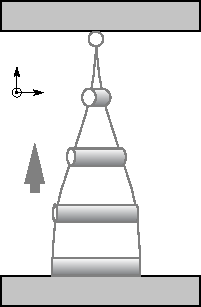
\includegraphics[scale=1.2]{figures/freedericksz_a.pdf}};
                \node at (-2.35,1.25) {$x$}; 
                \node at(-1.2,1.5) {$y$};
                \node at (-2.1,2.4) {$z$};
                \node at (-1.55,0.6) {$\vec{U}^\star$}; 
            \end{tikzpicture} 
        	\caption{Pixel "off" state}
        	\label{allume}
        \end{subfigure}	
        \begin{subfigure}[b]{0.49\textwidth}
        	\center
            \begin{tikzpicture}[scale=0.8]
                \node at (0,0) {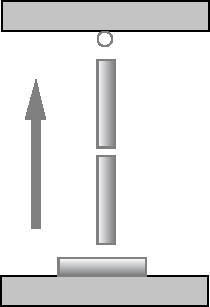
\includegraphics[scale=1.2]{figures/freedericksz_b.pdf}};
                \node at (-1.6,2.2) {$\vec{U}^\star$}; 
            \end{tikzpicture} 
        	\caption{Pixel "on" state}
        	\label{etteint}
        \end{subfigure}	
        
        \label{freedericksz} 
    \end{figure}

\center
Diagram of a LCD pixel using \textit{twisted nematic} technology.
\end{frame}
%%%%%%%%%%%%%

%%%%%%%%%%%%% 
\begin{frame}{Molecules orientation}
\framesubtitle{\ }
    \begin{figure}[h!]
    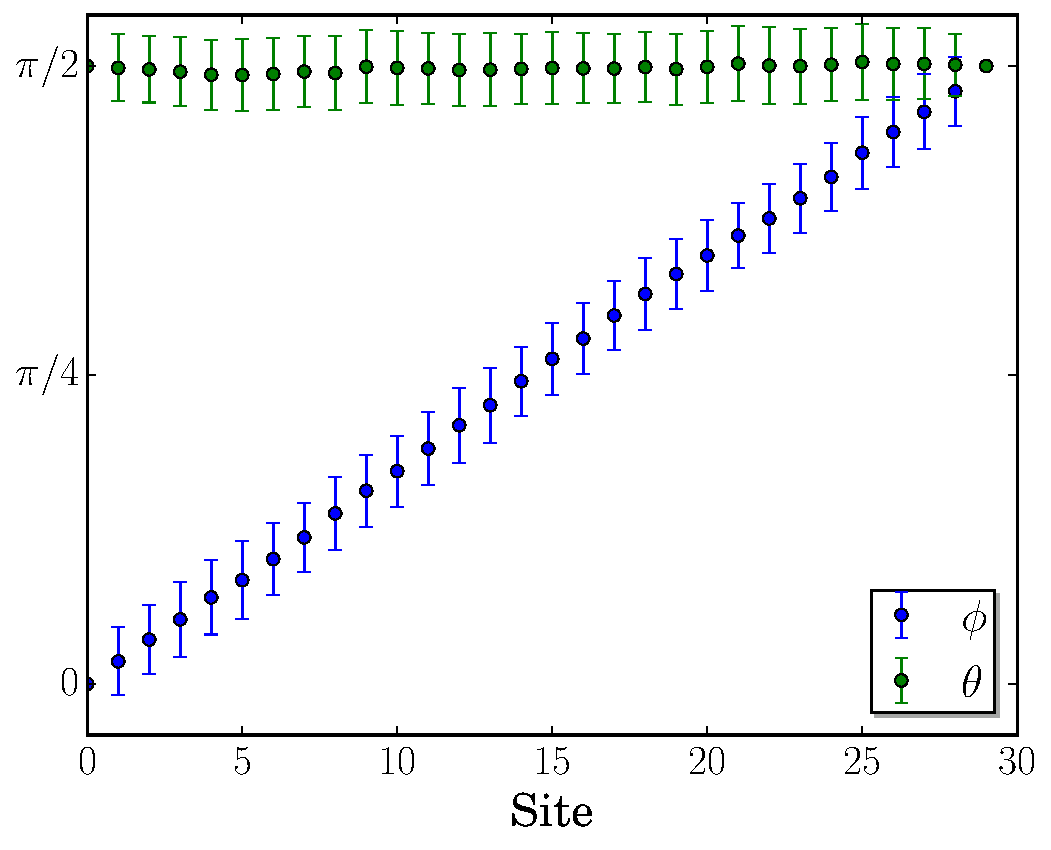
\includegraphics[scale=0.45]{figures/lcd_allume_T01.pdf}
    \end{figure}

\center
Molecule orientation \textbf{without} electric field
\end{frame}
%%%%%%%%%%%%%

%%%%%%%%%%%%% 
\begin{frame}{Molecules orientation}
\framesubtitle{\ }
    \begin{figure}[h!]
    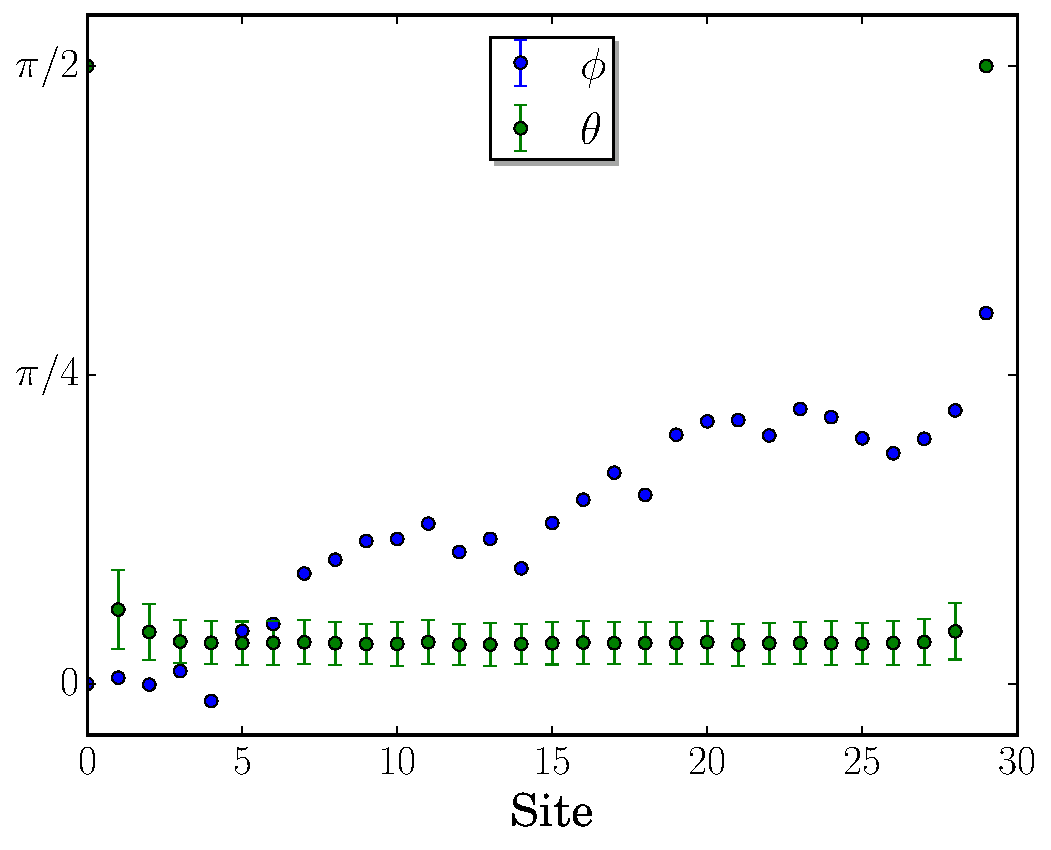
\includegraphics[scale=0.45]{figures/lcd_etteind.pdf}
    \end{figure}
\center
Molecule orientation \textbf{with} electric field
\end{frame}
%%%%%%%%%%%%%


%%%%%%%%%%%%% 
\begin{frame}
	\frametitle{Conclusion}
	\framesubtitle{\ }
    \only<2->{Detailed study of nematic-isotropic transition with Lebwohl-Laser model :
    \begin{itemize}
    \item first order transition at  $T^\star = 1.1232 \pm 0.0005$
    \end{itemize}}
    \only<2>{\center 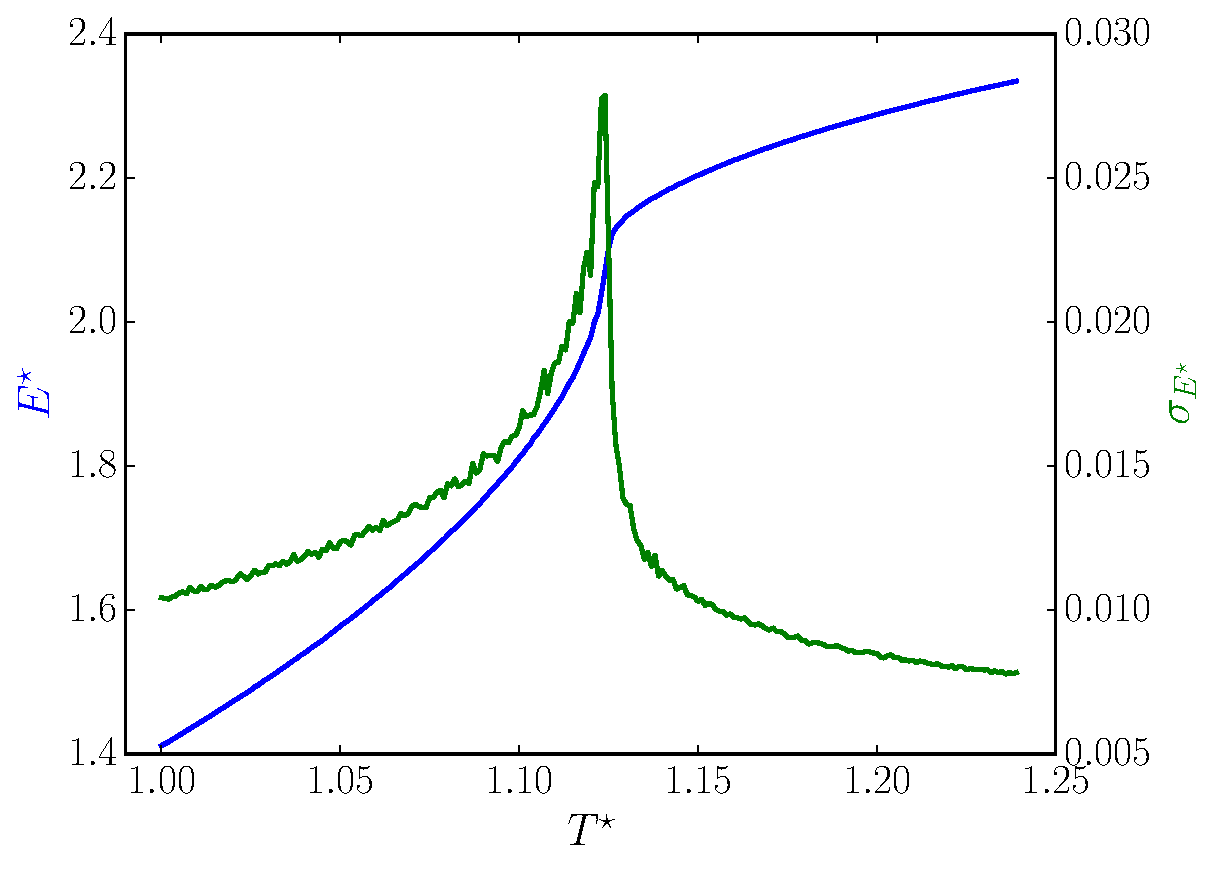
\includegraphics[scale=0.4]{figures/local_energie.pdf}}
    \only<3->{
    Electric field influence :
    \begin{itemize}
        \item shifts transition temperature and critical point for strong fields
    \end{itemize}
    }
    \only<3>{\center 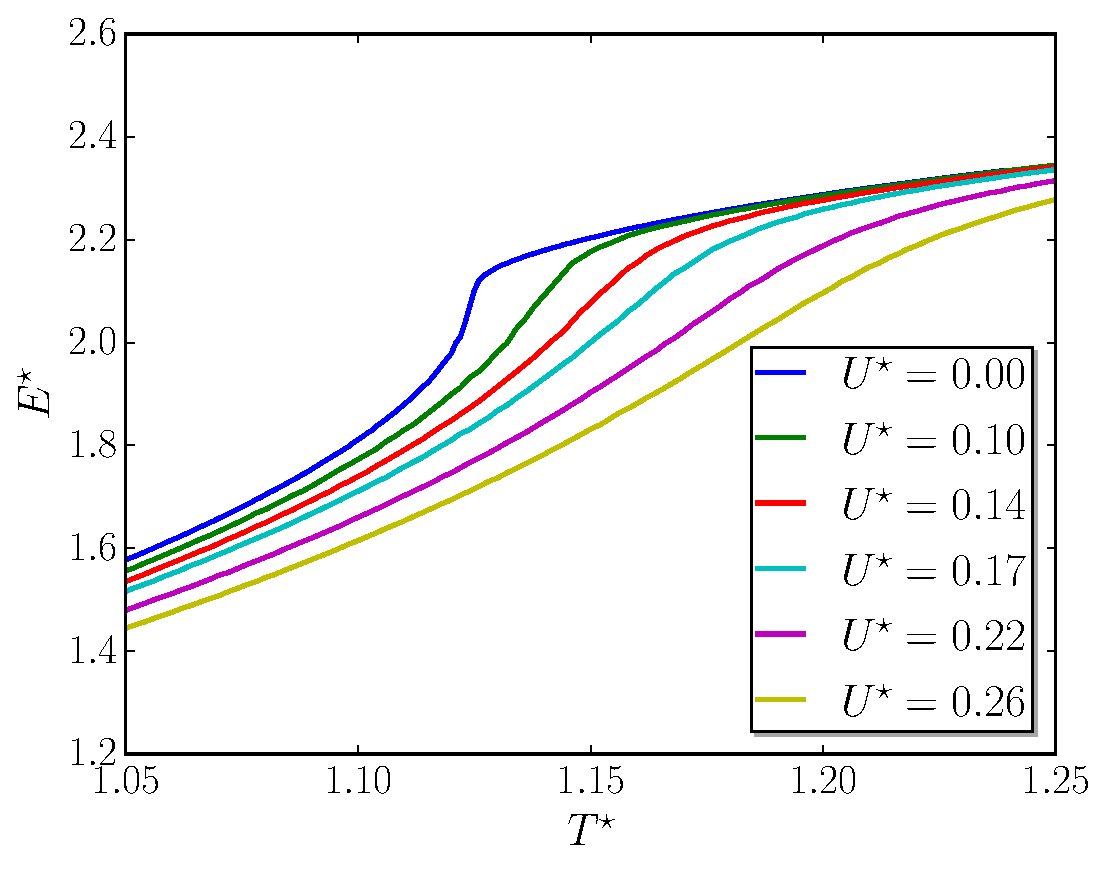
\includegraphics[scale=0.33]{figures/electricField_calo.pdf}}
    \only<4->{
    LCD and Fréedericksz :
    \begin{itemize}
        \item Lebwohl-Laser model can be used to model a LCD pixel
    \end{itemize}
    }
    \only<4>{
    \begin{figure}[h!]
    \center
        \begin{subfigure}[b]{0.49\textwidth}
        	\center
            \begin{tikzpicture}[scale=0.45]
                \node at (0,0) {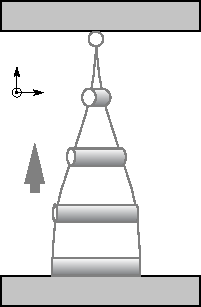
\includegraphics[scale=0.65]{figures/freedericksz_a.pdf}};
                \node at (-2.35,1.25) {$x$}; 
                \node at(-1.2,1.5) {$y$};
                \node at (-2.1,2.4) {$z$};
                \node at (-1.55,0.6) {$\vec{U}^\star$}; 
            \end{tikzpicture} 
        	\label{allume}
        \end{subfigure}	
        \begin{subfigure}[b]{0.49\textwidth}
        	\center
            \begin{tikzpicture}[scale=0.45]
                \node at (0,0) {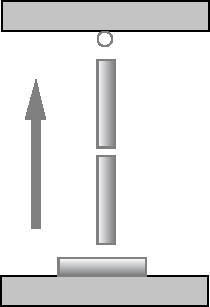
\includegraphics[scale=0.65]{figures/freedericksz_b.pdf}};
                \node at (-1.6,2.2) {$\vec{U}^\star$}; 
            \end{tikzpicture} 
        	\label{etteint}
        \end{subfigure}	
        
        \label{freedericksz} 
    \end{figure}
    }


\end{frame}
%%%%%%%%%%%%%

%%%%%%%%%%%%% 
\begin{frame}
	\frametitle{Perspectives}
	\framesubtitle{\ }
    Perspectives :
    \begin{itemize}
        \item Find the value of the critical field in that Fréedericksz transition 
        \item Study the temperature dependence of that transition
    \end{itemize}

\end{frame}
%%%%%%%%%%%%%

%%%%%%%%%%%%% 
\begin{frame}
	\frametitle{\ }
	\framesubtitle{\ }

{\center $\qquad$ \Huge Merci pour votre attention}

\end{frame}
%%%%%%%%%%%%%

%%%%%%%%%%%%% 
\begin{frame}
	\frametitle{yolo}
	\framesubtitle{\ }


\end{frame}
%%%%%%%%%%%%%


%%%%%%%%%%%%%
\end{document}